\chapter{LEAN SOFTWARE DEVELOPMENT}
\label{cha:lean}

Não é possível falar do desenvolvimento de \textit{software} enxuto (ou \textit{lean software development}) sem antes falar do sistema de produção criado pela Toyota e que deu origem ao \textit{lean}. Esse capítulo tem como objetivo aprofundar o leitor sobre a metodologia \textit{lean} de desenvolvimento de \textit{software} e dar uma introdução de seu surgimento na manufatura até sua utilização no desenvolvimento de \textit{software} conforme \citeonline{poppendieck:07}.
\label{lean}
\section{INTRODUÇÃO}

O sistema Toyota de produção, que deu origem ao \textit{lean}, surgiu como uma alternativa ao modelo de produção em massa aplicado por Henry Ford em 1914. Henry Ford conseguiu, através da produção em massa, aumentar o salário de 2,4 dolares por 9 horas de trabalho para 5 dolares por 8 horas de trabalho diário. Tudo isso foi conseguido através da redução de 85\% do trabalho sobre a produção do carro e da redução de 12 horas para apenas 90 minutos na sua produção, a qual passava através de uma linha de montagem com trabalho especializado. Nenhum trabalhador precisava saber fazer um carro inteiro, sendo necessário apenas treinar o funcionário para executar um tipo de trabalho na linha de produção. No sistema fordista de produção, o trabalho passou a ser essencialmente especializado e feito por qualquer tipo de pessoa, que poderia ser subtituída facilmente. Esse sistema de produção em massa demonstrou ser viável durante um certo tempo, mas apresentou problemas como a dificuldade de adaptação do modelo em relação a complexidade, que pode ser corroborada pela seguinte frase atribuída a Ford: ``O cliente pode ter o carro da cor que quiser, contanto que seja preto''. No modelo de produção em massa, o custo de uma mercadoria é reduzido de 15\% até 25\% conforme o número de unidades dobra, porém o custo de produção sobe de 20\% para 35\% cada vez que a variedade dobra.

O sistema de produção da Toyota apresenta vários conceitos e ideias que possibilitaram melhorar o sistema de produção e deixar as empresas mais competitivas como o fluxo JIT (\textit{Just in Time}) e o Jidoka (Autonomia). O fluxo JIT nada mais é do que eliminar o estoque e repensar o processo de produção em pequenos lotes. De modo prático, no sistema fordista tinha-se uma máquina especializada em fazer apenas uma peça do carro em massa, já no sistena da Toyota uma máquina poderia ser adaptada rapidamente para fazer diferentes partes rapidamente. O Jidoka, ou autonomia implantou a ideia de qualidade, fazendo com que qualquer evento anormal no processo de produção fizesse com que a produção fosse interrompida automaticamente, o que eliminava desperdício. O sistema deve ser projetado então para ser a prova de falhas, sem necessidade de um humano testando ou supervisionando para detectar erros, ou seja ele é isento de inspeção.

\section{LEAN}

A palavra \textit{lean}, empregada hoje, foi resultado da nova atribuição dada pelo livro lançado em 1990 e entitulado \textit{The Machine That Changed The World} para o que era chamado de JIT (\textit{Just-in-Time}) ou sistema Toyota de produção. Depois de seu lançamento, o que antes era chamado de sistema de produção Toyota passou a ser chamar produção enxuta ou \textit{Lean Production}. No início houve muita aversão ao emprego desse novo modelo de produção, mas conforme o tempo passou o pensamento \textit{lean} atingiu sucesso e foi empregado da manufatura para outras  áreas como: cadeia de suprimentos, desenvolvimento de produtos e no desenvolvimento de \textit{software}. A Figura \ref{fig:lean_tree} mostra a extensão do modelo \textit{lean} para outras áreas através da árvore da família \textit{lean}.

\begin{figure}[htb!]
\begin{center}
\caption{Árvore da família \textit{lean}}
\label{fig:lean_tree}
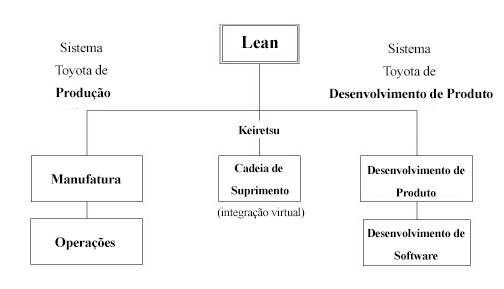
\includegraphics[width=11cm]{assets/lean_tree} \\
\fonte{\citeauthoronline{poppendieck:07}, \citeyear{poppendieck:07}.}
\end{center}
\end{figure}

Na área de manufatura, por exemplo, há o exemplo da companhia Dell de computadores que consegue entregar computadores customizáveis dentro de poucos dias. No que tange a cadeia de suprimentos, não adianta uma empresa ser \textit{lean} se os fornecedores da qual ela depende não forem. No exemplo da Dell, as empresas envolvidas na cadeia de produção do computador aprendem como trabalhar além da fronteira da empresa para alinhar seus interesses com a cadeira inteira de suprimentos. A manufatura enxuta e desenvolvimento enxuto compartilham certas características, o que torna fácil seu emprego no desenvolvimento de produto como redução no tempo de manufatura e redução no tempo de desenvolvimento. O \textit{software} nada mais é do que o desenvolvimento de um produto, sendo o desenvolvimento apenas um subconjunto de todo o processo. Nesse sentido, não há como melhorar a capacidade de desenvolvimento sem melhorar e entender o que constitui o desenvolvimento eficaz de um produto. Por isso, os princípios que regem o sistema Toyota de produção e o sistema Toyota de desenvolvimento são os mesmos. Os princípios do \textit{lean} para o desenvolvimento de \textit{software} são vistos a seguir.

\section{OS PRINCÍPIOS DO \textit{LEAN} NO DESENVOLVIMENTO}

A seguir são vistos os princípios do \textit{lean} no contexto do desenvolvimento de \textit{software} que são: 

\begin{itemize}
	\item Eliminação de desperdício;
	\item Incorporar qualidade;
	\item Criar conhecimento;
	\item Adiar compromisso 
	\item Entregar rápido
	\item Respeitar as pessoas e
	\item Otimizar o todo.
\end{itemize}

\subsection{Eliminação de Desperdício}
\label{sec:desperdicios}
O princípio da eliminação de desperdício é relacionado a tudo que não agrega valor para o cliente. No desenvolvimento de \textit{software} é importante entender o que significa esse valor, o qual pode mudar pelo fato dos clientes nem sempre saberem o que querem. Após entender esse desperdício, é preciso saber enxergá-lo dentro da organização. No desenvolvimento tudo que interfere no sentido de impedir que os usuários recebam esse valor ou qualquer atraso para que isso ocorra é considerado desperdício. Um exemplo comum de desperdício no desenvolvimento são funcionalidades extras. Segundo \citeonline{poppendieck:07} apenas 20\% das funcionalidades extras são usadas regularmente. Essas funcionalidades são basicamente coisas que não foram planejadas no início do desenvolvimento, mas que fazem com que a complexidade e manutenção do código se tornem custosa (além de testes desnecessários). Numa situação como essa, a empresa pode estar potencialmente gastando bastante com suporte e manutenção de funcionalidades que não agregam valor, ao invés de investir em coisas realmente úteis. Um mito que existe no desenvolvimento é que quanto mais cedo a especificação ocorrer, menor será o desperdício. Isso não é verdade, especialmente porque o cliente quase sempre não sabe o que precisa. Um escopo de funcionalidades que o sistema potencialmente pode ter pode ficar extenso e sofrer bastante modificações. 

A real motivação por trás da emilinação de desperdício é descobrir e eliminar desperdícios que podem reduzir custos e tornar os produtos mais efetivos. A Tabela \ref{tab:desperdicio} mostra a equivalência dos desperdícios na manufatura e no desenvolvimento de \textit{software}. Mais abaixo, é descrito um pouco sobre cada um desses desperdícios.

\begin{table}[htb!]
\centering
\caption{Os Sete Desperdícios}
\label{tab:desperdicio}
\vspace{0.5cm}
\begin{tabular}{l|l}

\hline                                
\textbf{Manufatura} & \textbf{Desenvolvimento de Software} \\ 
\hline                               
Estoques no processo & Trabalho parcialmente realizado \\
Superprodução & Funcionalidades extras \\
Excesso de Processamento & Reaprendizagem \\
Transporte & Transferência de controle \\
Movimentação & Troca de Tarefas \\
Esperas & Atrasos\\
Defeitos & Defeitos \\                               
\end{tabular}
\fonte{\citeauthoronline{poppendieck:07}, \citeyear{poppendieck:07}.}
\end{table}

Alguns exemplos de trabalhos parcialmente realizados podem ser: códigos não testados, códigos não documentados, códigos não mandados para ambiente de deploy (possivelmente por apresentarem conflitos na hora de mergear com outra \textit{branch}) etc.

O pior desperdício de todos é o de funcionalidades extras, o qual remete a funcionalidades que não são necessárias para entrega do trabalho ao cliente. Se não houver uma razão clara ou necessidade economica, essa funcionalidade não deve ser desenvolvida.

A questão de reaprendizagem se refere a toda vez seja descoberto algum conhecimento que já foi aplicado anteriormente, mas que foi reaprendido. Uma alternativa para esse problema é aplicar técnicas de gestão de conhecimento na organização e no desenvolvimento.

A transferência de controle tange na dificuldade de comunicação de conhecimento tácito, ou seja todo aquele que é adquirido pela experiência e que é difícil de se adquirir através de documentação. 

A troca de tarefas é um desperdício que acontece quando os desenvolvedores precisar trocar de uma tarefa para outra. Pode acontecer também de acontecer quando se tenta fazer mais de uma tarefa ao mesmo tempo. O planejamento das tarefas por um gestor de projetos pode eliminar esse problema com a aplicação de métodos como caminho crítico etc.

O atraso e defeitos são os outros problemas comuns de desperdício e que estão relacionados com o mal uso dos recursos humanos ou planejamento errado e falta de investimento em testes de prevenção.

\subsection{Incorporar Qualidade}
\label{sec:quality}

Esse princípio do \textit{lean} no desenvolvimento de \textit{software} está relacionado com a incorporação de qualidade no código desde o início. Assim, o teste não deve ser feito apenas no final do processo de desenvolvimento. A inspeção no processo de qualidade deve-se dar principalmente antes que o defeito ocorra (controlando todas as condições de ambiente necessárias). 
No desenvolvimento de \textit{software} existem técnicas como o TDD (\textit{Test Driven Development}) para resolver esse problema de qualidade. 	
O TDD tem seu início com a escrita do SUnit, uma biblioteca de testes, em Smalltalk por Kent Beck nos anos 90. Seu uso era encorajado para facilitar a execução de testes de \textit{software} automatizados, que eram feitos de forma manual até então. Posteriormente houve a criação do SUnit para Java (chamado de JUnit) juntamente com Erich Gamma. Mais tarde houve a portabilidade para outras linguagens como Ruby, Python, C++, Perl e Php.\footnote{O padrão da família formada pela portabilidade dessa biblioteca de teste para todas as linguagens se chama SUnit.}. Com o amadurecimento das bibliotecas SUnit, essa ferramenta deixou de servir apenas como uma forma de automatização de testes e passou a ser utilizada principalmente para atividades de \textit{design} do código. O TDD é uma prática de desenvolvimento que envolve criar testes antes de escrever o código que será testado. Nela, o desenvolvedor escreve um pequeno trecho de teste para um código que ainda não existe. O desenvolvedor depois roda o teste, e naturalmente ele falha. Depois disso, o desenvolvedor apenas escreve código suficiente para que o teste passe. \cite{barauna:13}

A vantagem de escrever os testes antes do código de produção é que ao final do desenvolvimento tem-se um código testado e que serve como uma documentação viva do sistema. Toda vez que seja preciso fazer uma modificação no sistema ou adição de novas funcionalidades, os testes são executados e, caso essa nova funcionalidade afete o comportamente do que já foi testado, o teste falha, o que ajuda na liberação de funcinalidades que possuem menos probabilidade de dar problema em produção. A Figura \ref{fig:tdd} mostra o ciclo \textit{red -- green -- refactor} utilizado no TDD. Primeiramente o desenvolvedor escreve um código que falhe. Depois disso, ele faz o teste passar. Quando o teste passar, ele melhora o código para torná-lo mais legível. A ideia de fazer o código falhar é entender e projetar o código aos poucos. Quando se procede dessa maneira, pode-se descobrir todos os casos possíveis de um problema e assim, os códigos ficam melhores e menos propensos a erros.

\begin{figure}[htb!]
\begin{center}
\caption{Ciclo red -- green -- refactor}
\label{fig:tdd}
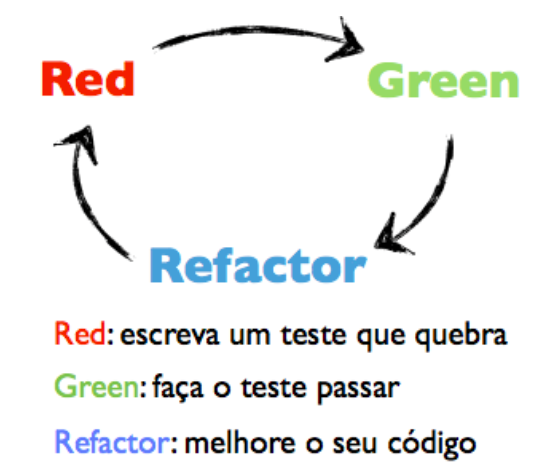
\includegraphics[width=9cm]{assets/tdd} \\
\fonte{\citeauthoronline{barauna:13}, \citeyear{barauna:13}.}
\end{center}
\end{figure}	

Outra abordagem para incorporar qualidade é o BDD (\textit{Behavior Driven Development}) que é uma evolução do TDD. O BDD começou como uma tentativa de melhor entender e explicar o processo do TDD. O problema era basicamente a palavra ``Teste'' no TDD que fazia com que os desenvolvedores não utilizassem o TDD como uma ferramente de \textit{design} ou projeto para o \textit{software}. Com o passar do tempo, o BDD evoluiu no sentido de testar o comportamento de um objeto ao invés de sua estrutura interna (como é o foco do TDD). \cite{chelimsky:12}


A Figura \ref{fig:bdd} ilustra o processo do BDD. Primeiramente o desenvolvedor descreve um cenário de teste. Após a escrita desse cenário, é escrita uma \textit{step-definition}, que descreve um comportamento de uma funcionalidade do sistema. Nessa \textit{step-definition}, o desenvolvedor escreve somente o um trecho de código necessário para o teste falhar. Após esse processo, entra-se num ciclo do BDD que foi mostrado anteriormente. Na linguagem ruby pode-se utilizar o Cucumber e o Rspec como \textit{frameworks} para BDD e TDD respectivamente.

\begin{figure}[htb!]
\begin{center}
\caption{Ciclo do BDD}
\label{fig:bdd}
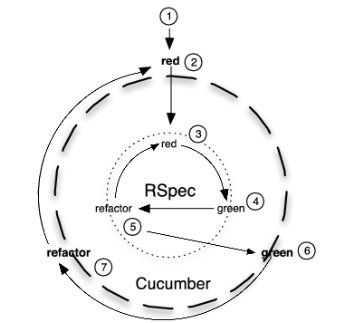
\includegraphics[width=9cm]{assets/bdd} \\
\fonte{\citeauthoronline{chelimsky:12}, \citeyear{chelimsky:12}.}
\end{center}
\end{figure}	

O trabalho do teste não pode-se limitar apenas a encontrar defeitos de produção no sistema e sim fazer  que os erros e problemas posssam ser previnidos e detectados para que não entrem em produção.

\subsection{Criar Conhecimento}

O conhecimento do desenvolvimento de \textit{software} não é criado em apenas uma etapa. Um dos problemas com o modelo de desenvolvimento em cascata (visto na sessão \ref{sec:cascata}) é que ele assume que todo conhecimento é adquirido na etapa de análise, porém a construção de um \textit{software} é um processo de criação de conhecimento. Mesmo que todos os detalhes sejam vistos na etapa de análise, os detalhes de \textit{design} sempre ocorrem na etapa de contrução (quando o \textit{software} está sendo codificado). Um processo de desenvolvimento que seja focado na criação de conhecimento deve esperar que o \textit{design} evolua durante a codificação, principalmente porque o cliente quase sempre não sabe o que quer, assim o \textit{feedbacks} dos \textit{stakeholders} são importantes nesse processo e dão direcionamento para o que está sendo elaborado.

As empresas que possuem excelência no desenvolvimento de \textit{software} aprendem no processo de construção do \textit{software} e utilizam o conhecimento aprendido para futuros projetos. O processo de desenvolvimento precisa encorajar o aprendizado através do ciclo de desenvolvimento. 


\subsection{Adiar Compromisso}

Um sistema de \textit{software} é passivel de sofrer mudanças: todos os requisitos e riscos dificilmente vão ser mitigados em uma primeira etapa de análise. Porém, toda e qualquer decisão que torne o processo de mudança mais difícil ou irreverssível deve ser postergada até o último momento. É melhor deixar uma decisão importante para o último momento do que tomar uma decisão prematura que não leve a lugar algum. Isso não significa que todas as decisões devem ser postergadas, o time ou o líder de tecnologia deve comprometer-se a fazer com que a maioria das decisões sejam reversíveis com um sistema e arquitetura que sejam o mais flexível possível. As vezes a pressa pela eliminação de riscos a fim de diminuir a incerteza pode levar a decisões erradas que são irreversíveis. O melhor a se fazer é experimentar várias soluções, deixando as opções em aberto para serem tomadas o mais tarde possível com os testes e avaliações necessários.

\subsection{Entregar rápido}

Todo desenvolvimento de \textit{software} deve ser feito da forma mais rápida possível para que o cliente não tenha tempo de mudar de ideia. Num mundo rápido e cada vez mais competitivo, a rapidez de implementação de uma ideia pode ser fundamental para seu sucesso. Isso pode ser conseguido através da eliminação do desperdício e gastos desnecessários, diminuição das taxas de erros (através de inspeções no código) etc.

A teoria das filas é uma teoria que pode ajudar nesse sentido. Muitas vezes no desenvolvimento há novas demandas de cliente ou defeitos para serem corrigidos e organizar essas é de certa maneira desafiador. A teoria das filas ajuda no gerenciamento dessa lista de ``requisitos''.

\subsection{Respeitar pessoas}

Três dos quatro pilares do sistema de desenvolvimento de produtos da Toyota dizem respeito as pessoas envolvidas no processo de desenvolvimento de um produto. Assim, esse é um princípio muito importante que norteia o desenvolvimento \textit{lean}.

As pessaos são motivadas a trabalharem em produtos de sucesso e para conseguir-se produtos de sucesso é necessário bons líderes. Empresas que respeitam seus empregados desenvolvem grandes líderes que por sua vez são capazes de conduzir grandes projetos. Além disso, é necessário assegurar-se que o conhecimento técnico necessário esteja presente na pessoa que designa a função. Distrubuir a pessoa de acordo com seu perfil e capacidade para um projeto é fundamental para o sucesso do projeto. O respeito as pessoas está relacionado com a capacidade do time em se organizar em relação aos planos e objetivos da empresa. Todas as pessoas precisam fazer parte do processo: isso envolve desenvolvedores, \textit{stakeholders} etc. O processo de construção de \textit{software} também é um processo de certa forma ``social''.

\subsection{Otimizar o todo}

Uma empresa que utiliza-se do \textit{lean} otimiza a cadaia de valor desde o princípio até seu final. Se algum processo dentro dessa cadeia não é otimizado, o processo como um todo é afetado. Aqui é feita uma análise do processo de desenvolvimento \textit{lean}, mas não adianta o processo de desenvolvimento ser otimizado, se outros processos que também fazem parte do processo de negócio apresentarem deficiência. Uma das ferramentas presentes e que foi mostrado no Capítulo 1 é a utilização de mapas de cadeia de valor. Através da análise da cadeia de valor é possível enxergar desperdícios com uma visão holistica de todo o processo da empresa. 

\section{DISCIPLINA, QUALIDADE e 5S}

No desenvolvimento de \textit{software} \textit{lean} não é possível acelerar o desenvolvimento sem incorporar qualidade no produto (como foi visto nos princípios do \textit{lean} acima). Para tornar-se \textit{lean} é indispensável que haja disciplina no que diz respeito a maneira como o \textit{software} é desenvolvido. Ao entrar em ambiente de desenvolvimento é possível perceber o nível de disciplina que uma equipe possui. Se a sala de desenvolvimento está bagunçada, possívelmente a equipe é desleixada, o que pode fazer com que o código também possua essa qualidade negativa. O Cinco S é uma ferramenta clássica do \textit{lean} que ajuda a organizar o espaço de trabalho de uma equipe garantindo que tudo que seja necessário esteja em mãoes no momento que a equipe precise. Os Cinco S são referências as palavras japonesas \textit{seiri, seiton, seiso, seiketsu e shitsuke}. Essas palavras foram traduzidas para a língua inglesa e são: \textit{sort} (organização), \textit{sistematize} (classificação), \textit{shine} (limpeza), \textit{standardize} (padronização) e \textit{sustain} (autodisciplina). No desenvolvimento de \textit{software}, o 5S não se aplica apenas ao ambiente físico, mas também ao ambiente lógico por trás da tela. Para organização poderia ser, por exemplo, remover e fazer \textit{backup} de códigos e arquivos que não são mais utilizados, para classificação envolve organizar as coisas nos servidores de forma que o ambiente possa ser utilizado por qualquer pessoa da empresa. Limpeza pode ser manter o ambiente de desenvolvimento limpo (sem copos, marcas de dedo na tela etc.). Padronização envolve, por exemplo, colocar automatização para garantir que cada estação de trabalho tenha a versão mais recente ou a que foi acordada para o desenvolvimento do produto, \textit{backup regular} etc. A autodisciplina só precisa ser então mantida no ambiente. 


Em \citeonline{poppendieck:07} é mostrado também os 5S em relação a linguagem Java, mas que serve para a programação em geral. Abaixo é mostrado cada S com sua respectiva ação para melhoria.

\subsection{Organização}
\label{lean:org}

A organização na linguagem Java envolve reduzir o tamanho do código do repositório. Para isso, é necessário eliminar tudo que for:

\begin{itemize}
	\item Códito morto (que não faz nada);
	\item Imports que não são utilizados;
	\item Variáveis que não são utilizadas;
	\item Métodos que não são utilizados;
	\item Classes que não são utilizadas e
	\item Refatorar códigos redundantes.
\end{itemize}

\subsection{Classificação}

A classificação ou sistematização envolve organizar o projeto e pacotes. Tudo precisa ter uma local e tudo precisa estar no seu devido lugar. Para isso é necessário:

\begin{itemize}
	\item Resolver ciclos de dependência de pacotes e
	\item Minimizar depenpências.
\end{itemize}

\subsection{Limpeza}

Os problemas são mais visíveis quando o código está limpo e claro. Para resolver problemas de limpeza pode-se executar as seguintes ações:

\begin{itemize}
	\item Resolver testes que estão falhando e erros;
	\item Melhorar cobertura de código;
	\item Melhorar performance de teste e
	\item Resolver os ``\textit{warnings}'' que aparecem no teste ou nos \textit{logs}.
\end{itemize}

\subsection{Padronizar}

Uma vez que o ambiente encontra-se limpo, deve-se mantê-lo asssim. Reduzir a complexidade é importante para melhorar o processo de manutenção. Uma técnica bastante utilizada para resolver questões desse tipo é médir o \textit{software}. Primeiramente é necessário saber o que medir e para quê. Esses dados são importantes e podem dar uma direção para equipe no que tange a qualidade do código. Uma técnica de medição, chamada de complexidade ciclomática pode ajudar segundo \citeonline{laird:06}. Quanto maior a complexidade do código, mais difícil é mantê-lo.

\subsection{Autodisciplina}

Para autodisciplina é necessário seguir e usar procedimentos.


\section{CONCLUSÃO DO CAPÍTULO}

Nesse capítulo foi visto sobre a metodologia \textit{lean} de desenvolvimento. O \textit{lean} foi uma metodologia de desenvolvimento que nasceu na manufatura e que hoje está cada vez mais sendo aplicada no \textit{software}. Foram visto os princípios do \textit{lean} como eliminação de desperdícios, incorporar qualidade, criar conhecimento, adiar compreomisso, entregar rápido, repeitar pessoas e otimizar o todo e como eles são aplicados no desenvolvimento. A importância de testes e detecção de falhas também foi explicada. Além disso, foi discutida a importância do mapeamento do fluxo de valor para uma empresa de forma a entender e eliminar os despedícios. Utilizar uma prática do \textit{lean} não necessáriamente vai tornar uma empresa \textit{lean} se os desperdícios não forem eliminados e o processo não for melhorado. Sem fazer esse mapeamento do fluxo de valor, não há como melhorar o processo. No próximo capítulo são mostradas algumas melhorias que foram identificas e até implementadas no que diz respeito aos princípios do \textit{lean}. 
